\documentclass[11pt]{article}

\usepackage[utf8]{inputenc}
\usepackage[margin=1in]{geometry}
\usepackage[english]{babel}
\usepackage{tocloft}
\usepackage{amsmath}
\usepackage{amsfonts}
\usepackage{amssymb}
\usepackage[none]{hyphenat}
\usepackage{graphicx}
\usepackage{fancyhdr}
\usepackage{pdfpages}
\usepackage{glossaries}
%\usepackage{setspace}
%\usepackage{tikz}
\usepackage[font={small,it}]{caption}

\parindent 0ex
\linespread{1.5}
\setlength{\headheight}{30pt}
\setcounter{tocdepth}{1}
\pagestyle{fancy}

\fancyhead{}
%\fancyfoot{}
\fancyhead[L]{\slshape \MakeUppercase{Binarization of the Minutes of the Early Synod \newline Meetings of the Reformed Churches of South-Africa}}
\rhead{
\includegraphics[width=3.7cm, height=1.2cm]{nwulogo.jpeg}}

\makeglossaries

\newglossaryentry{GNOME}{name=GNOME, description={GNU Network Object Model Environment}}
\newglossaryentry{GHz}{name=GHz, description={Gigahertz}}

\begin{document}
	%insert pdf cover page
	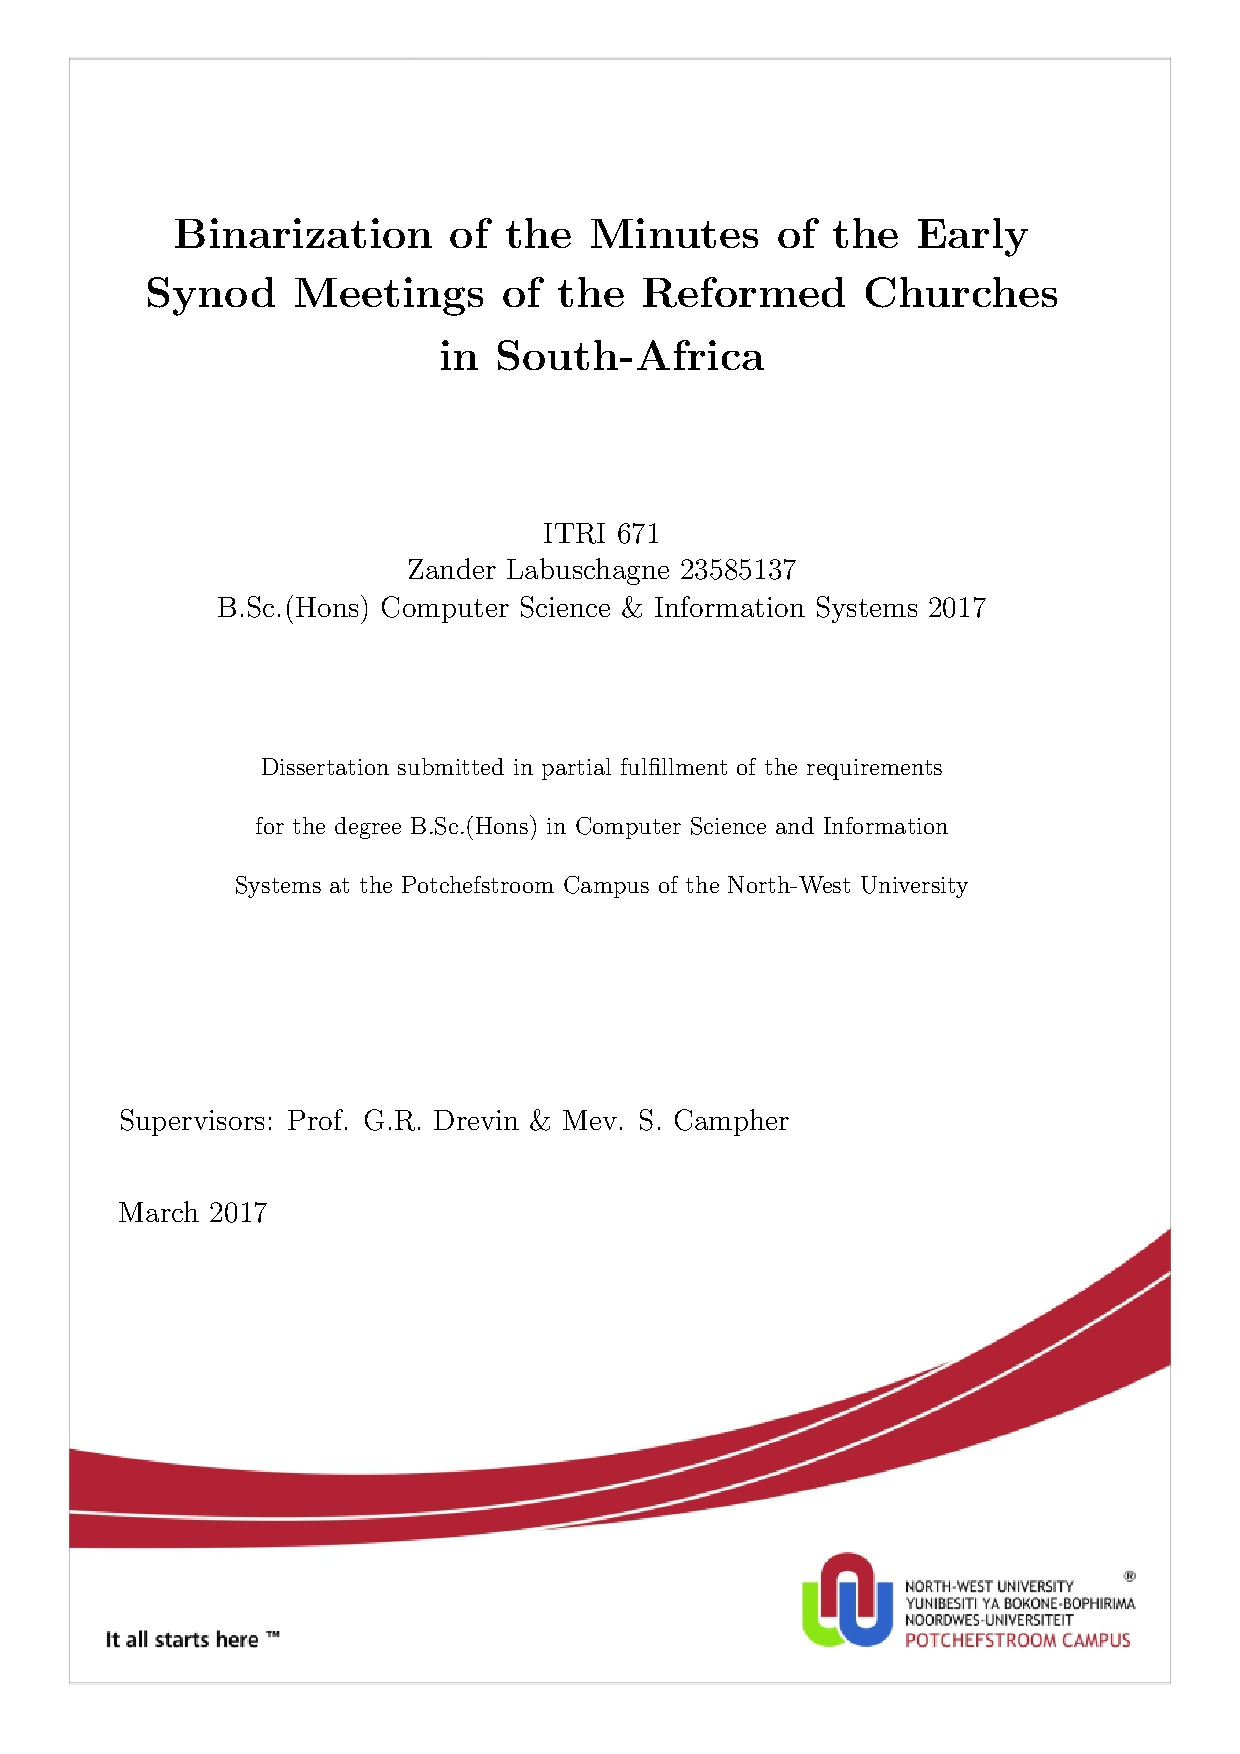
\includepdf[pages={-},offset=0mm 0mm, width=21.5cm, height=28cm]{Cover.pdf}

    \renewcommand{\cftsecleader}{\cftdotfill{\cftdotsep}} % TOC Dotted Lines
    \tableofcontents
    \thispagestyle{empty}
    \clearpage

    \listoffigures
    \thispagestyle{empty}
    \clearpage

	%\printglossary[title=Abbreviation]

    \setcounter{page}{1}

	\section{Introduction} % 1-2p[0.5p] : Agtergrond : Rationale
		This project will determine the binarization algorithm(s) or combination of binarization algorithms which best preserves the quality of the text of historical handwritten document images, more specifically the document images containing the minutes of the early synod meetings of the Reformed Churches of South-Africa.\\

		The main contribution of this project will result in a detailed description of an algorithm which proved to be the best in terms of preserving the quality of historical handwritten document text, as well as the actual algorithm in Matlab syntax along with the proof supporting the solution's performance whether it be a comparison of binarized images or statistical data. The algorithm will also be implemented and used to binarize the document images mentioned earlier.

	\section{Problem Description} % [2.5p] -> Tekort/Probleem -> Navorsingsvraag/Probleemstelling
    % + Motivation, existing solutions + study contribution
    		\textit{If I had an hour to solve a problem I'd spend 55 minutes thinking about the problem and 5 minutes thinking about solutions.}\\
    		[-1.25cm]
    		\begin{flushright}
    			\textit{Albert Einstein}
		\end{flushright}

    	\subsection{Background}
    		The idea for this project came to mind when the Theological Library of the North-West University at the Potchefstroom Campus saw the need for the digitalization of historical documentation. The library realized that if nothing is done to prevent further degradation on their archives it will not last forever even in the carefullest hands. The greater picture is to digitalize all the archives in order to keep the history in tact even after the original documentation perishes completely, this will also in turn provide easier access to many more people who are interested in this information as well as providing easier and quicker search methods. However this project will currently focus on the binarization objective only.\\

    		Binarization in image processing is the process of discriminating the foreground from the background in an image by changing the foreground pixels or text to black and the background or paper pixels to white \cite{ntogas2008binarization}. Binarization is also considered by many computer scientists as a critical step in the processing of images because it has the greatest impact on the quality grade of all the processing that follows such as document analysis \cite{jacob2014survey}, thus a good binarization result would greatly improve the results of page-segmentation, optical character recognition and any other subsequent processing \cite{agrawal2011stroke}, while a bad binarization result will cause any following processing techniques to yield inadequate results \cite{howe2011laplacian}. A good binarization algorithm is one that best preserves the foreground and omit as much background as possible.\\

    		Other topics to be considered in this study which forms part of the binarization algorithm is the calculation of a threshold value, pre-processing and post-processing techniques which aims to increase the performance of the binarization algorithm and finally the evaluation of the binarization method at the end of the study to determine the successfulness of the algorithm.

    \subsection{Existing Research}
    		A considerable amount of binarization algorithms exist and they all have their advantages and disadvantages, some fit better for certain circumstances or for a certain type of image. No existing binarization algorithm is good to suit all types of images \cite{lins2015binarizing}, but one can improve the result by combining algorithms \cite{ntogas2008binarization}, by adding pre-processing and post-processing techniques to the binarization algorithm such as noise removal \cite{agrawal2011stroke}, \cite{lins2015binarizing}, or by careful experimentation and analysis on a very specific dataset in order to train the algorithm accordingly. One of the key objectives in binarization is thresholding, which is the calculation algorithm of the middle or ``split'' value used to discriminate the foreground from the background in the image. The algorithm would mark the pixels in a binary fashion and divide them into two categories, ON denoting the set of pixels representing the foreground or OFF denoting the set of pixels representing the background \cite{o1995document}.\\

    		There are some research going on in historical document processing as seen in the Historical document Imaging and Processing Proceedings, the research contained in the Historical document Imaging and Processing Proceedings documentation will probably be of good use during this project, but they mostly focus on character recognition or word spotting of foreign characters such as Arabic and Chinese writing. Another similar  application which is also more popular is the identification and characterization of the writer or author of historical documentation \cite{ogier2006madonne}. It seems that little focus is placed on the binarization of historical handwritten documents resulting in insufficient research \cite{jacob2014survey} which provides the opportunity to do more research in this field.\\

    		\newpage

    		Promising solutions are the combination of various binarization algorithms \cite{su2011combination}, as presented in the article with the title: Combination of Document Image Binarization Techniques, written by Su, Lu and Tan. and presented at the 2011 International Conference on Document Analysis and Recognition. It is probable that this approach would be the most successful since it was tested on historical documentation. Gatos's binarization algorithm also demonstrated promising results in an article named Adaptive Degraded Document Image Binarization, written by Gatos, Pratikakis and Perantonis\cite{gatos2006adaptive}, although these images weren't historical but degraded in a way that is comparable to historical documentation. The techniques presented in Binarizaing Complex Scanned Documents by Lins and Almeida \cite{lins2015binarizing} might also be considered since these techniques handle problems similar to those one encounter in historical document image processing. Other proven binarization algorithms includes Souvola's and Otsu's algorithms but have only been proven successful in good circumstances. The algorithms of Chen and Wang will also be considered during this research.\\

    		Existing Research also shows that pre-processing and post-processing techniques can greatly improve the binarization results \cite{jacob2014survey}, \cite{ntogas2008binarization}.

    \subsection{Rationale}
		The reason for this research project is that there is not many successful binarization algorithms capable of performing the task this problem requires, most algorithms are adequate in only the perfect circumstances such as on good quality documents \cite{jacob2014survey}, or adapted for a specific set of image types, but this project deals with degraded and historically written documentation which is very daunting to read even for human eyes. Other reasons accountable for the lack of success are the order of variations in degraded documentation, there are simply too many variations to generalize all under one class for one algorithm \cite{ntogas2008binarization}.

	\subsection{Problem Statement}
    		The problem statement is to determine and implement the binarization algorithm which best preserves the quality of the document images, specifically historical handwritten text on degraded paper. To preserve the quality of a document image is to extract the useful information with high accuracy from the image while omitting the background and irrelevant information. See \textit{Figure \ref{voorbeeld}} for an example of the document images to be binarized.

    		%Voorbeeld Figure
		\begin{figure}[h]
			\centering
			\includegraphics[scale=0.11]{DSC_0446.JPG}
			\caption{Example of document image to be binarized} % Figuur Naam
			\label{voorbeeld} % label om na figuur te verwys
		\end{figure}

	\section{Research Aims and Objectives} % 0.5p [1p]
		The aim of this study is to propose a binarization algorithm that bests differentiate the foreground(text, tables and figures) from the background(paper and stains) in historical handwritten documentation, specifically on the dataset which is the minutes of the early synod meetings of the Reformed Churches in South-Africa.\\

	The objectives to accomplish in order to achieve the above aim is to:
	\begin{itemize}
		\item Perform a literature study on thresholding techniques and binarization algorithms for grey scale images, handwritten documents and historical documentation. A small literature study will also be done on pre-processing and post-processing techniques for document binarization, it will be small because it is not very common to implement these extra processing techniques. It is also necessary to perform a literature study on the evaluation of document image binarization.
		\newpage
		\item Familiarization with MathWorks Matlab and/or the Matlab Image Processing Toolbox which will be used to test and analyse the thresholding, pre-processing and post-processing techniques and binarization algorithms, the design and implementation of the binarization algorithm will also be done in the Matlab environment at the end of the study.
		\item Analysis of the performance of existing thresholding techniques and binarization algorithms on the historical handwritten documents dataset. Experimenting with pre-processing and post-processing techniques will also be done to achieve maximum performance from the binarization algorithm.
		\item Improve existing binarization algorithm(s), combine existing binarization algorithms, incorporate other image processing techniques into existing binarization algorithms or design a new binarization algorithm if existing solutions yield totally inadequate binarization results.
		\item Evaluate and implement the final binarization algorithm(s) of choice.
	\end{itemize}

	\section{Procedures and Methods}%Google -> Vindicated???
		This section will discuss the research methodology as well as the procedures and methods that will be followed to finally conclude this research. The research methodology will shape the process this project will undergo and methods chosen when experimenting with solutions.

		\subsection{Research Paradigm}
			Research is defined as ``the creation of new knowledge using an appropriate process, to the satisfaction of the users of the research'' \cite{oates2005researching}. There are numerous reasons for doing research, the research conducted during this project has three reasons behind it, the first is to add to the body of knowledge. Since there aren't many successful binarization algorithms for the binarization of historical handwritten document images, this research will aim to provide the scientific community with an algorithm which is tested and proven to be the most effective for the binarization of historical handwritten document images. The second reason is to solve a problem, as stated in the problem description section this project is motivated to digitalize historical documentation and to solve the problem of the degradation and loss of information. The third reason behind this research is to come up with a better way, a better way of binarizing historical handwritten document images. The existing methods or binarization algorithms does not suffice as explained in the problem description section.\\

			Research usually concludes into something useful to someone. This research will result in a part-product, part-theory and a critical analysis. The theory may be completely new or may be a reinterpretation of an existing theory, this research might use existing theories or techniques in image processing and apply it in a different context, the word ``theory'' is used because it has yet to be tested and accepted in practice as well. The critical analysis will be the analysis of the binarization algorithms and the various techniques they incorporate.\\

			A research paradigm is a way of thinking about aspects of the world when doing research, three research paradigms exists, positivism, interpretivism and critical research of which positivism is the most commonly used paradigm. Interpretivism is a study where one tries to create and provide an understanding of how certain factors are related in a social context, therefore no hypothesis is required in the interpretivism philosophical paradigm. There exist no acceptable success criteria for the interpretivism paradigm. Critical research is concerned with the contradictions in the modern world and to aid in the elimination of alienation and domination. This research project will follow a positivism philosophical paradigm, which is an approach to research in the natural sciences. The positivism philosophical paradigm is also know as the scientific method \cite{oates2005researching} or the hypothetico-deductive method.\\

		%Epistomology, ~Ontology
			This research will follow the hypothetico-deductive methodology as explained by Dodig-Crnkovic, 2009. This methodology is found suitable for this research project because it is a scientific method for the study of natural sciences, and since this project mainly entails image processing which is a branch of computer science which originates from the fields of mathematics and logic which is both fields of the natural sciences \cite{tucker2004computer}. ``Computer science is the study of computational processes and information structures, including their hardware realizations, their linguistic models, and their applications'' \cite{tucker2004computer}. The scientific or hypothetico-deductive methodology is chosen as the research methodology. This methodology excels in this type of research because it evaluates the solutions through experimenting or the construction of prototypes, which is algorithms in the case of this research project \cite{dodig2002scientific}. \\

			The hypothetico-deductive methodology works on the assumptions that the world is ordered, regular and not random which one can investigate in an objective manner. Everything can be investigated objectively because everything is independent of human cognition. The hypothetico-deductive methodology can never be proven true, a scientist can only predict what should happen (with a certain probability) by using the knowledge concluded from a series of experiments \cite{oates2005researching}, but a good theory must always have the possibility of falsification. If the theory is not falsifiable, it should not be trusted, because a theory becomes trustworthy once it has been tested many times with failure to falsify.\\

			%Scientific Method Figure
			\begin{figure}[h]
				\centering
				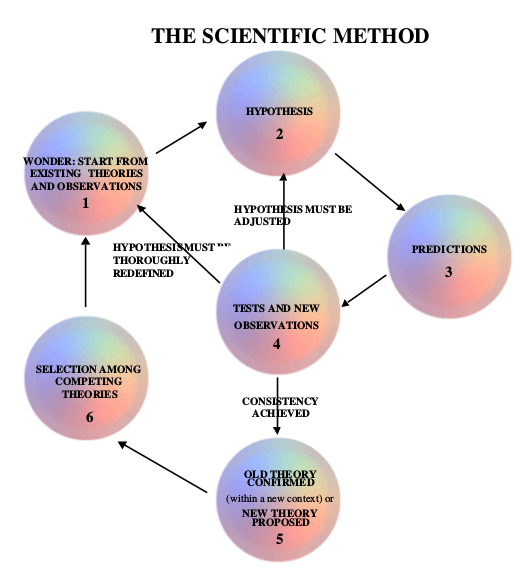
\includegraphics[scale=0.5]{scientific_method.png}
				\caption{The Scientific Method \textsc{\protect\cite{dodig2002scientific}}} % Figuur Naam
				\label{scientificmethod} % label om na figuur te verwys
			\end{figure}

			The hypothetico-deductive methodology follows a recursive series of six steps as explained below and shown in \textit{Figure \ref{scientificmethod}}:
			\begin{enumerate}
				\item Provide a research question or problem statement which can be answered or solved in terms of existing knowledge or one that requires a new theory.
				\item Formulate a hypothesis.
				\item Deduce consequences and make predictions.
				\item Conduct experiments to test the hypothesis objectively, existing science must accommodate the hypothesis. If the hypothesis contradicts existing science, the hypothesis must be refuted and careful testing must follow. Steps two through three is repeated until consistency is obtained.
				\item If consistency is obtained through enough iterations, the hypothesis becomes a confirmed theory.
				\item The new theory is compared to existing theories.
			\end{enumerate}%Verduidelik die metodologie

	Research methods of this study will include the following subsections.

	\subsection{Algorithm Performance Analysis}
		Performance analysis of algorithms will be done by experimenting and prototyping of the algorithms and by comparing and evaluating the binarization results. The algorithms will be tested on the minutes of the early synod meetings of the Reformed Churches in South-Africa dataset by using Matlab.

	\subsection{Algorithm Design}
		Modification of existing algorithms or the design of a new algorithm, if opportune, will also be done on Matlab as well as the implementation of the final algorithm that will be used to binarize the images in the previous mentioned dataset.

	\subsection{Binarization Result Evaluation}
		The results of the binarization will be evaluated by using the research done on evaluation as well as by comparison and inspection by the study leaders and/or other computer scientists.

	\subsection{Artefact}
		The resulting artefact will be a binarization algorithm with a step by step explanation of the algorithm, the Matlab code for the algorithm will also be provided as well as examples of the results produced by the algorithm to determine the successfulness of the algorithm. A prototyping development method will be used because a series of different prototypes(Matlab code and results) will be compared against each other and modifications to the algorithms will happen iteratively until the best performing algorithm is found.\\

		This project will be very similar to the project of Jacques B. Barnard's, the only difference is that the data of Barnard's project consists of printed text while the data of this project consists of handwritten text, with both texts containing similar content.

	\section{Approach to Project Management and Project Plan}
		As stated in the previous chapter, this project will follow an iterative prototyping development methodology. The work needed to be done for this project is defined in a series of deliverables that has to be completed and submitted on predefined dates as stated in the study guide for this module, ITRI 671. Each deliverable has its own objectives and requirements to be met. The work flow for this project will be presented as a Gantt chart created with Planner 0.14.6, a project management application for the \gls{GNOME} desktop. This Gantt chart will be used throughout the research term to maintain the project's time schedule.\\

		%Gantt Chart Figure
		\begin{figure}[h]
			\centering
			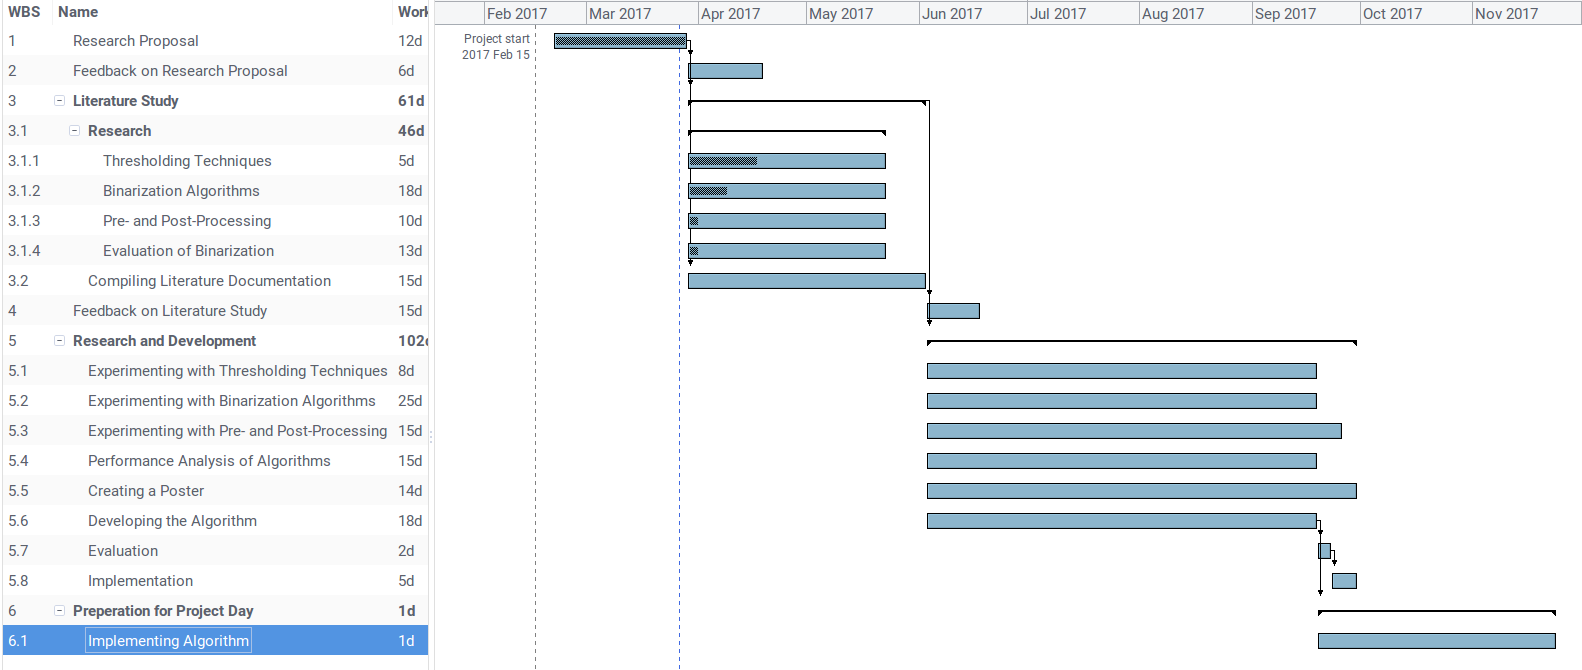
\includegraphics[scale=0.29]{Gantt.png}
			\caption{Project Gantt Chart} % Figuur Naam
			\label{gantt} % label om na figuur te verwys
		\end{figure}

		This project commenced on the 15\textsuperscript{th} of February 2017 and will finish on the 23\textsuperscript{rd} of November 2017. The following milestones are important for the success and time management of this project. Submission of the project proposal, this document, will be on the 27\textsuperscript{th} of March 2017 at 17:00. Students get feedback from supervisors about their project proposals on the 18\textsuperscript{th} of April 2017. The literature study will be submitted on the 2\textsuperscript{nd} of June 2017. All students will get feedback from supervisors about their literature study on the 17\textsuperscript{th} of July 2017. The artefact or final product that this research study has concluded to will be demonstrated on the 29\textsuperscript{th} of September 2017 along with a poster summarizing the research study. The submission of the complete set of documentation will be on the 23\textsuperscript{rd} of October 2017. There will be a project day on the 23\textsuperscript{rd} of November 2017 where all project will be on display as well as presentations about the projects.\\

		Fortunately this research project requires no additional financing and all equipment and software that'll be necessary for this research project to succeed are paid for and available. There are no additional costs to research since the university already has loads of documentation and information, and the natural sciences library will purchase any additional information with the inter library loans if requested.

		\subsection{Scope}
			As stated in the Introduction chapter this project is only concerned with the binarization aspect of the broader aim of this project. The binarization will consist of the calculation of a threshold value and might include pre-processing and post-processing techniques as well. The binarization algorithm will be specifically chosen, improved or designed and implemented only for the minutes of the early synod meetings of the reformed churches in South-Africa, which is handwritten text on degraded paper but may not perform as well on other types of documentation.

		\subsection{Risks}
			The only risk this projects entails is the risk of damaging the historical archives of the theological library while scanning the documentation. Some precautions are taken to keep this risk to a minimum such as wearing cotton gloves when handling the documentation and using a tweezers to lift a page. The documentation is also handled with extra care when paging and scanning and folding the pages is prohibited.

	\section{Development Platform, Resources and Environments}
		The environment will be strictly scientific because this project is of no interest in an economical environment nor has it economic purposes. The final implementation will only be used once, the results or processed data will be presented to users or community thereafter. The research, experience and knowledge gathered will be well documented and shared to become of use to other computer scientists who seeks to achieve similar goals for the sole purpose to broaden the knowledge of the scientific community.\\

	A personal computer(MSI GE62VR-6RF Apache Pro Laptop) will be used for processing since the processing does not require an industrial level of processing. The computer has an Intel Core i7 6700HQ processor with 4 cores and 8 threads running at a clock speed of 2.6\gls{GHz} utilizing 8GB of DDR4 RAM and a nVidia GeForce GTX 1060 with 6GB of GDDR5 RAM. The screen on which the binarized images will be compared on is a 15" MSI LCD IPS panel with a resolution of 1920x1080. The computer and hardware are of sufficient quality and has the performance capabilities suitable to satisfy all requirements necessary in order to accomplish the goals of this project. Processing will be done via MathWorks Matlab and/or the Matlab Image Processing Toolbox since the software will only be used for scientific purposes and not for consumer nor commercial use. Matlab started out as a matrix laboratory many years ago, today it is a mathematical tool for mathematicians and scientists used to perform complex calculations at a large scale. Matlab contains all the functions and features necessary to overcome all objectives required to achieve the aim of this project. The personal computer is running an operating system called Zorin OS Ultimate, with generic Linux kernel 4.8.0-41 and Gnome/Zorin Desktop Environment. \LaTeX \space in conjunction with \TeX maker will be used for all documentation because of its simplicity, accuracy, neatness and the ease of use of \TeX maker, the resulting document will be presented in PDF format because PDF is used very widely and highly compatible with many systems.\\

	Other resources that'll be used includes the MathWorks Matlab help documentation and numerous books on Matlab such as Introduction to Matlab and Simulink - A project Approach 3\textsuperscript{rd} Ed., 2008 by Beucher and Weeks; Matlab - A Practical Introduction to Programming and Problem Solving 3\textsuperscript{rd} Ed., 2013; Matlab for Dummies, 2015 by Sizemore and Mueller; Matlab Programming Fundamentals R2015a, 2015; and Practical Image and Video Processing Using Matlab, 2011 by Oge Marques.

	\section{Ethical and Legal Implications}
		This project has only one ethical implication because no people not related to this project will be affected during the research term. The only ethical implication is that the research conducted is original and that no plagiarism is involved. The only legal implications are the use of software in a legal fashion. The MathWorks Matlab software and all toolboxes are used with an academic license obtained from the North-West University. Word processing software being used for the documentation such as this document are the \LaTeX \space libraries and the \TeX maker \LaTeX \space interface which is being used under the free GNU General Public License version 2. The operating system being used is Zorin OS Ultimate which is paid for in full by the author of this document. Any other operating systems which might be used are other Linux distributions such as Manjaro which is free to use and also released under the GNU General Public License version 2.

    \section{Provisional Chapter Division}
    	\subsection{Introduction}
    		The introduction will include a description of the project, the aim of the project along with the objectives to be completed in order to achieve the aim of this project. The introduction chapter will also include a background a a rationale. The methods of investigation will also be discussed in this chapter.

    	\subsection{Research Methodology}
    		The research methodology chosen for this project will be discussed as well as the reasons for choosing this methodology.

    	\subsection{Literature Study}
    		This chapter will contain the literature study on the research topics at hand, namely a small part on the research methodology, thresholding techniques, followed by binarization algorithms as well as pre-processing and post-processing techniques and finally the evaluation of binarization algorithms in order to determine the successfulness of the proposed algorithms.

    	\subsection{Threshold Calculation}
    		The method of calculation for the threshold will be discussed here as well as the justifications for using the proposed calculation(s).

    	\subsection{Evaluation of Binarization Algorithms}
    		Binarization algorithms will be evaluated in this chapter  and compared against each other. The combination of binarization algorithms will be evaluated in this chapter as well.

    	\subsection{Pre- and Post-Processing Techniques}
    		Pre- and post-processing techniques that forms part of the binarization algorithm will be explained in this section.

    	\subsection{Design/Implementation of Binarization Algorithm}
    		The implementation of the proposed binarization algorithm or combination of algorithms will be explained in this chapter. The design of a new binarization algorithm will also be explained if necessary and possible.

    	\subsection{Results}
    		The result of the proposed algorithm(s) or solution will be demonstrated in this chapter in order to determine the successfulness of the algorithm. The results will either be presented as binarized images for visual inspection or in a table containing statistical data to compare the successfulness of the algorithm to other existing algorithms.

    	\subsection{Conclusion}
    		The conclusion derived from the research done will be presented in this chapter as well as future research and improvements needed to be done.

    	\subsection{Reflection}
		A summary of the research study accomplishments will be given in this chapter along with the student's views and reflection about this project.

    \newpage
    \bibliographystyle{plain}
    \bibliography{ref}
    \addcontentsline{toc}{section}{{}References}
    \thispagestyle{plain}
    \clearpage

    \section*{Appendix A: Research Proposal}
    \addcontentsline{toc}{section}{{}Appendix A: Research Proposal}
    %\pagenumbering{gobble}
    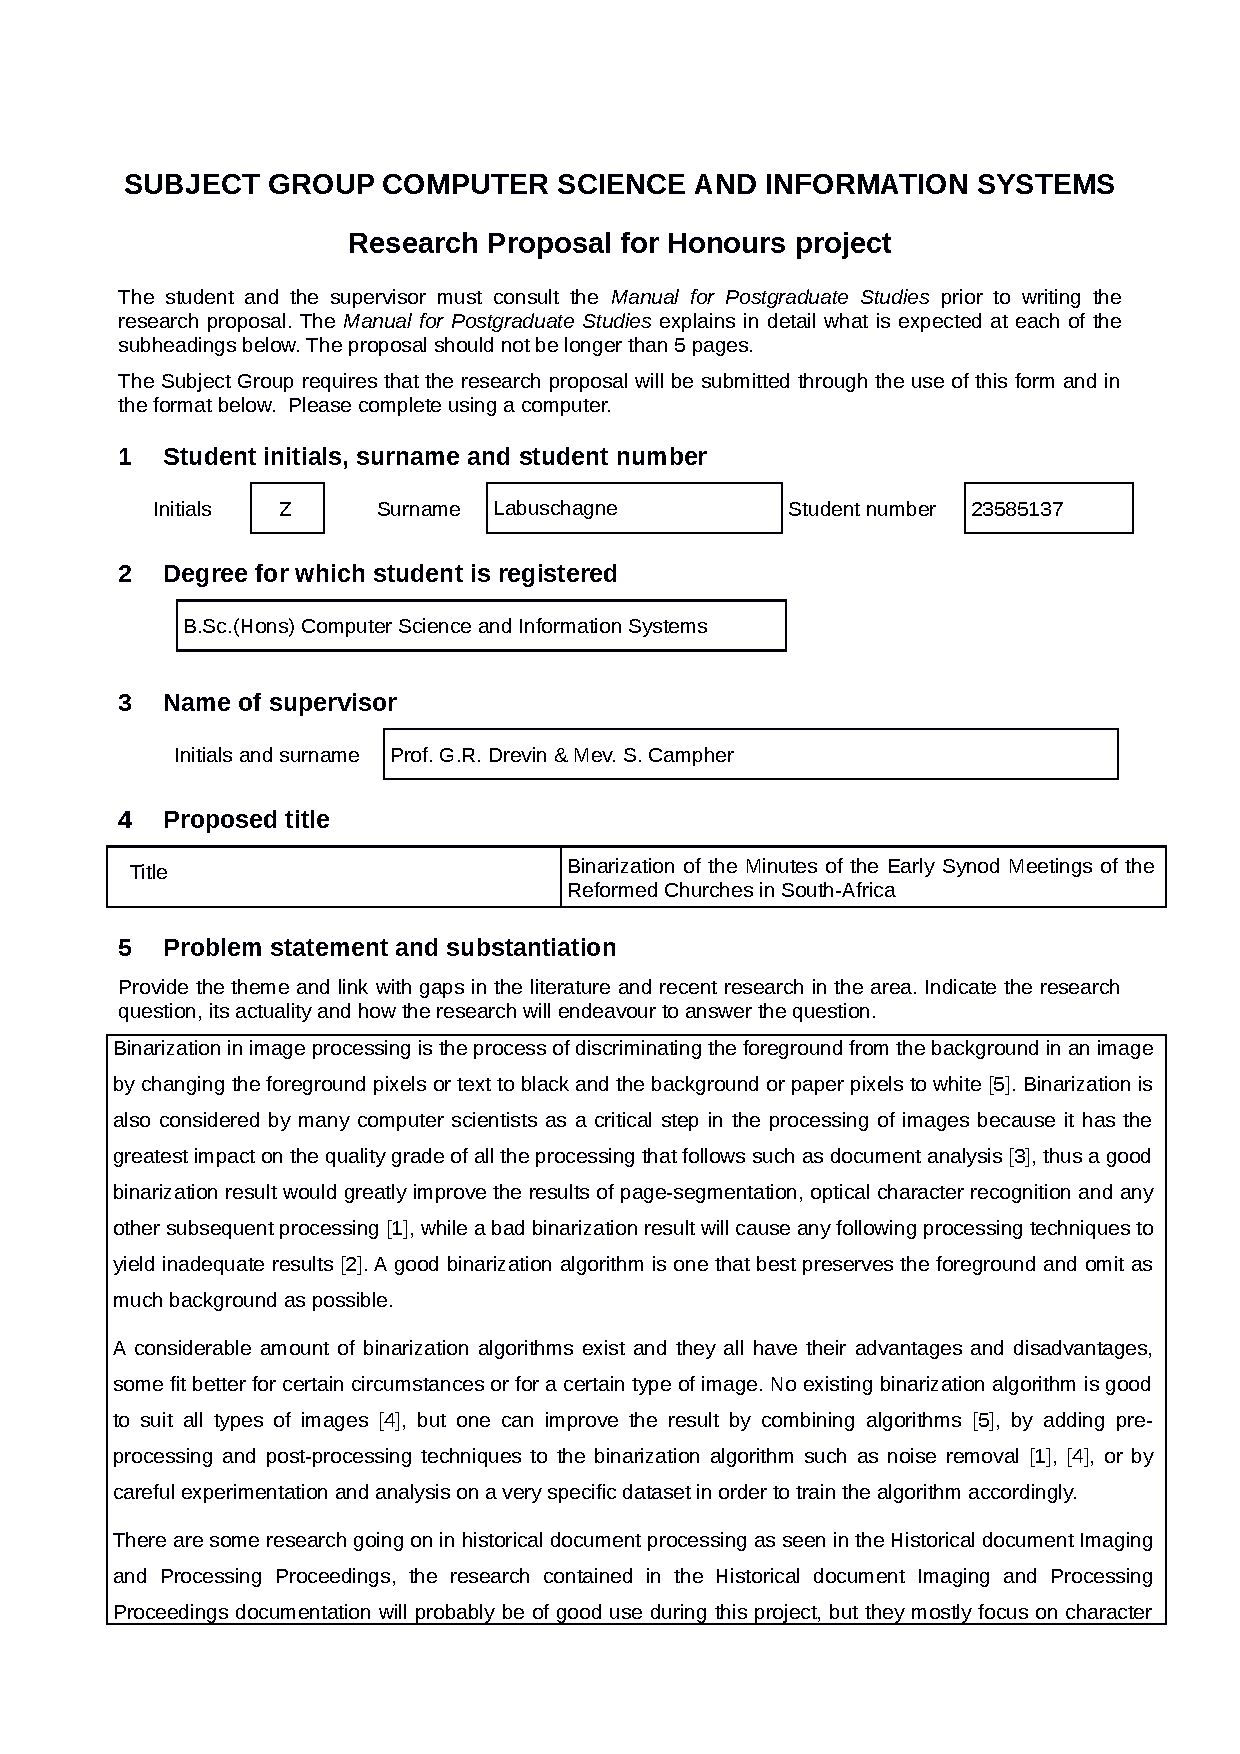
\includepdf[pages={-},offset=0mm 0mm, width=21.5cm, height=28cm]{Appendix_A.pdf}

\end{document}
